\chapter{排序}

\section{插入排序} %%%%%%%%%%%%%%%%%%%%%%%%%%%%%%


\subsection{直接插入排序}
\textbf{直接插入排序}(Straight Insertion Sort)的基本思想是:把数组a[n]中待排序的n个元素看成为一个有序表和一个无序表,开始时有序表中只包含一个元素a[0],无序表中包含有n-1个元素a[1]~a[n-1],排序过程中每次从无序表中取出第一个元素,把它插入到有序表中的适当位置,使之成为新的有序表,这样经过n-1次插入后,无序表就变为空表,有序表中就包含了全部n个元素,至此排序完毕。在有序表中寻找插入位置是采用从后向前的顺序查找的方法。

直接插入排序的C语言实现如下。
\begin{Codex}[label=straight_insertion_sort.c]
/** 数组元素的类型 */
typedef int elem_t;

/**
  * @brief 直接插入排序,时间复杂度O(n^2).
  *
  * @param[inout] a 待排序元素序列
  * @param[in] start 开始位置
  * @param[in] end 结束位置,最后一个元素后一个位置,即左闭右开区间
  * @return 无
  */
void straight_insertion_sort(elem_t a[], const int start, const int end) {
    elem_t tmp;
    int i, j;

    for (i = start + 1; i < end; i++) {
        tmp = a[i];
        for (j = i - 1; tmp < a[j] && j >= start; j--) {
            a[j + 1] = a[j];
        }
        a[j + 1] = tmp;
    }
}
\end{Codex}


\subsection{折半插入排序}
在查找插入位置时,若改为折半查找,就是\textbf{折半插入排序}(Binary Insertion Sort)。

折半插入排序的C语言实现如下。
\begin{Codex}[label=binary_insertion_sort.c]
/**
  * @brief 折半插入排序,时间复杂度O(nlog2n).
  *
  * @param[inout] a 待排序元素序列
  * @param[in] start 开始位置
  * @param[in] end 结束位置,最后一个元素后一个位置
  * @return 无
  */
void binary_insertion_sort(elem_t a[], const int start, const int end) {
    elem_t tmp;
    int i, j, left, right, mid;

    for (i = start + 1; i < end; i++) {
        tmp = a[i];
        left = start;
        right = i - 1;
        while (left <= right) {
            mid = (left + right) / 2;
            if (tmp < a[mid]) {
                right = mid - 1;
            } else {
                left = mid + 1;
            }
        }
        for (j = i - 1;j >= left; j--) {
            a[j + 1] = a[j];
        }
        a[left] = tmp;
    }
}
\end{Codex}


\subsection{希尔(Shell)插入排序}
从对直接插入排序的分析得知,其算法时间复杂度为$O(n^2)$,但是,若待排序记录序列为“正序”时,其时间复杂度可提高至$O(n)$。由此可设想,若待排序记录序列按关键字“基本有序”,即序列中具有下列特性
$$R_i.key < \max\left\{R_j.key\right\},\; j<i$$
的记录较少时,直接插入排序的效率就可大大提高,从另一方面来看,由于直接插入排序算法简单,则在n值很小时效率也比较高。希尔排序正是从这两点分析出发对直接插入排序进行改进得到的一种插入排序方法。

\textbf{希尔排序}(Shell Sort)的基本思想是:设待排序元素序列有n个元素,首先取一个整数$gap=\lfloor \dfrac{n}{3} \rfloor+1$作为间隔,将全部元素分为gap个子序列,所有距离为gap的元素放在同一个子序列中,在每一个子序列中分别施行直接插入排序。然后缩小间隔gap,取$gap=\lfloor \dfrac{gap}{3}\rfloor+1$ ,重复上述的子序列划分和排序工作,直到最后取$gap=1$,将所有元素放在同一个序列中排序为止。

图~\ref{fig:shellsort}展示了希尔排序的过程。

\begin{center}
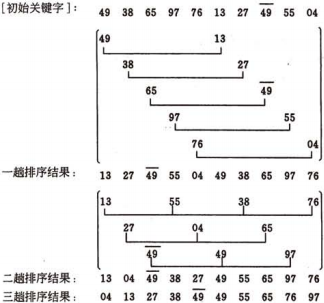
\includegraphics[width=240pt]{shellsort.png}\\
\figcaption{希尔排序}\label{fig:shellsort}
\end{center}

希尔排序的C语言实现如下。
\begin{Codex}[label=shell_sort.c]
/*
  * @brief 一趟希尔插入排序.
  *
  * 和一趟直接插入排序相比,仅有一点不同,就是前后元素的间距是gap而不是1
  *
  * @param[inout] a 待排序元素序列
  * @param[in] start 开始位置
  * @param[in] end 结束位置,最后一个元素后一个位置,即左闭右开区间
  * @param[in] gap 间隔
  * @return 无
  */
static void shell_insert(elem_t a[], const int start, const int end, const int gap) {
    elem_t tmp;
    int i, j;
    for (i = start + gap; i < end; i++) {
        tmp = a[i];
        for (j = i - gap; tmp < a[j] && j >= start; j -= gap) {
            a[j + gap] = a[j];
        }
        a[j + gap] = tmp;
    }
}

 /*
  * @brief 希尔排序.
  * @param[inout] a 待排序元素序列
  * @param[in] start 开始位置
  * @param[in] end 结束位置,最后一个元素后一个位置,即左闭右开区间
  * @return 无
  */
void shell_sort(elem_t a[], const int start, const int end) {
    int gap = end - start;
    while (gap > 1) {
        gap = gap / 3 + 1;
        shell_insert(a, start, end, gap);
    }
}
\end{Codex}


\section{交换排序} %%%%%%%%%%%%%%%%%%%%%%%%%%%%%%


\subsection{冒泡排序}
\textbf{冒泡排序}(Bubble Sort)的基本方法是:设待排序元素序列的元素个数为n,从后向前两两比较相邻元素的值,如果发生逆序(即前一个比后一个大),则交换它们,直到序列比较完。我们称它为一趟冒泡,结果是最小的元素交换到待排序序列的第一个位置,其他元素也都向排序的最终位置移动。下一趟冒泡时前一趟确定的最小元素不参加比较,待排序序列减少一个元素,一趟冒泡的结果又把序列中最小的元素交换到待排序序列的第一个位置。这样最多做n-1趟冒泡就能把所有元素排好序。

冒泡排序的C语言实现如下。
\begin{Codex}[label=bubble_sort.c]
/** 数组元素的类型 */
typedef int elem_t;

/**
  * @brief 冒泡排序.
  * @param[inout] a 待排序元素序列
  * @param[in] start 开始位置
  * @param[in] end 结束位置,最后一个元素后一个位置,即左闭右开区间
  * @return 无
  * @note 无
  * @remarks 无
  */
void bubble_sort(elem_t a[], const int start, const int end) {
    int exchange; /* 是否发生交换*/
    elem_t tmp;
    int i, j;

    for (i = start; i < end - 1; i++) {
        exchange = 0;
        for (j = end - 1; j > i; j--) { /* 发生逆序,交换*/
            if (a[j - 1] > a[j]) {
                tmp = a[j - 1];
                a[j - 1] = a[j];
                a[j] = tmp;
                exchange = 1;
            }
        }
        if (exchange == 0) return; /* 本趟无逆序,停止处理*/
    }
}
\end{Codex}

\subsection{快速排序}
\textbf{快速排序}(Quick sort)的基本思想是任取待排序元素序列中的某个元素(例如取第一个元素)作为基准,按照该元素的关键字大小,将整个元素序列划分为左右两个子序列:左侧子序列中所有元素的关键字都小于基准元素的关键字,右侧子序列中所有元素的关键字都大于或等于基准元素的关键字,基准元素则排在这两个子序列中间(这也是该元素最终应该安放的位置)。然后分别对这两个子序列重复施行上述算法,直到所有的元素都排在相应位置为止。

一趟快排的过程如图~\ref{fig:bubblesort} (a)所示。整个快速排序的过程可递归,如图~\ref{fig:bubblesort} (b)所示。

\begin{center}
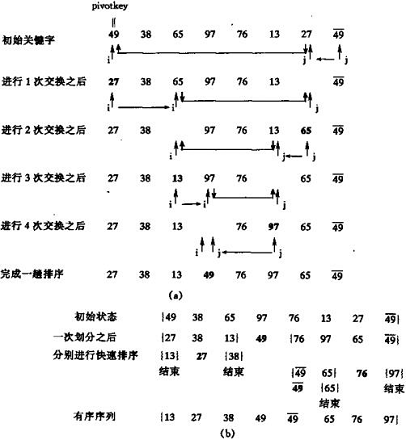
\includegraphics{bubblesort.png}\\
\figcaption{快速排序示例}\label{fig:bubblesort}
\end{center}

更多详细解释请参考本项目的wiki,\myurl{https://github.com/soulmachine/acm-cheatsheet/wiki/快速排序}

快速排序的C语言实现如下。
\begin{Codex}[label=quick_sort.c]
/** 数组元素的类型 */
typedef int elem_t;
 /*
  * @brief 一趟划分.
  * @param[inout] a 待排序元素序列
  * @param[in] start 开始位置
  * @param[in] end 结束位置,最后一个元素后一个位置,即左闭右开区间
  * @return 基准元素的新位置
  */
int partition(elem_t a[], const int start, const int end) {
    int i = start;
    int j = end - 1;
    const elem_t pivot = a[i];

    while(i < j) {
        while(i < j && a[j] >= pivot) j--;
        a[i] = a[j];
        while(i < j && a[i] <= pivot) i++;
        a[j] = a[i];
    }
    a[i] = pivot;
    return i;
}

/**
  * @brief 快速排序.
  * @param[inout] a 待排序元素序列
  * @param[in] start 开始位置
  * @param[in] end 结束位置,最后一个元素后一个位置
  * @return 无
  */
void quick_sort(elem_t a[], const int start, const int end) {
    if(start < end - 1) { /* 至少两个元素*/
        const int pivot_pos = partition(a, start, end);
        quick_sort(a, start, pivot_pos);
        quick_sort(a, pivot_pos + 1, end);
    }
}
\end{Codex}


\section{选择排序} %%%%%%%%%%%%%%%%%%%%%%%%%%%%%%
\textbf{选择排序}(Selection sort)的基本思想是:每一趟在后面n-i(i=1, 2, ..., n-2)个元素中选取最小的元素作为有序序列的第i个元素。


\subsection{简单选择排序}
\textbf{简单选择排序}(simple selection sort)也叫直接选择排序(straight selection sort),其基本步骤是:
\begindot
\item 在一组元素a[i]~a[n-1]中选择最小的元素;
\item 若它不是这组元素中的第一个元素,则将它与这组元素的第一个元素对调;
\item 在剩下的a[i+1]~a[n-1]中重复执行以上两步,直到剩余元素只有一个为止。
\myenddot

简单选择排序的C语言实现如下。
\begin{Codex}[label=simple_selection_sort.c]
/** 数组元素的类型 */
typedef int elem_t;

/**
  * @brief 简单选择排序.
  * @param[inout] a 待排序元素序列
  * @param[in] start 开始位置
  * @param[in] end 结束位置,最后一个元素后一个位置,即左闭右开区间
  * @return 无
  */
void simple_selection_sort(elem_t a[], int start, int end) {
    elem_t tmp;
    int i, j, k;

    for (i = start; i < end; i++) {
        k = i;
        /* 在a[i]到a[end-1]中寻找最小元素*/
        for (j = i + 1; j < end; j++)
            if(a[j] < a[k]) k = j;
        /* 交换*/
        if (k != i) {
            tmp = a[i];
            a[i] = a[k];
            a[k]= tmp;
        }
    }
}
\end{Codex}


\subsection{堆排序}
堆排序的C语言实现如下。
\begin{Codex}[label=heap_sort.c]
#include "heap.c"
/**
  * @brief 堆排序.
  * @param[inout] a 待排序元素序列
  * @param[in] n 元素个数
  * @param[in] cmp cmp 比较函数,小于返回-1,等于,大于
  * @return 无
  */
void heap_sort(heap_elem_t *a, const int n, 
               int (*cmp)(const heap_elem_t*, const heap_elem_t*)) {
    int i;
    heap_t *h;
    heap_elem_t tmp;

    h = heap_create(n, cmp);
    h->elems = a;

    i = (h->size - 2)/2;   /* 找最初调整位置:最后分支结点*/
    while (i >= 0) {  /* 自底向上逐步扩大形成堆*/
        heap_sift_down(h, i);
        i--;
    }

    for (i = h->size - 1; i > 0; i--) {
        tmp = h->elems[i];
        h->elems[i] = h->elems[0];
        h->elems[0] = tmp;
        h->size = i; /* 相当于h.size -- */
        heap_sift_down(h, 0);
    }
    heap_destroy(h);
}
\end{Codex}


\section{归并排序} %%%%%%%%%%%%%%%%%%%%%%%%%%%%%%
所谓“归并”,就是将两个或两个以上的有序序列合并成一个有序序列。我们先从最简单的二路\textbf{归并排序}(Merge sort)入手。

图~\ref{fig:mergesort}是一个二路归并排序的例子。

\begin{center}
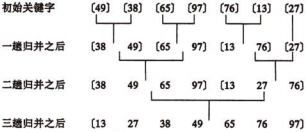
\includegraphics{mergesort.png}\\
\figcaption{二路归并排序示例}\label{fig:mergesort}
\end{center}

二路归并排序的C语言实现如下。
\begin{Codex}[label=merge_sort.c]
/** 数组元素的类型 */
typedef int elem_t;

 /** 数组元素的类型 */
typedef int elem_t;

 /*
  * @brief 将两个有序表合并成一个新的有序表
  * @param[inout] a 待排序元素序列,包含两个有序表
  * @param[in] tmp 与a等长的辅助数组
  * @param[in] start a[start]~a[mid-1]为第一个有序表
  * @param[in] mid 分界点
  * @param[in] end a[mid]~a[end-1]为第二个有序表
  * @return 无
  */
static void merge(elem_t a[], elem_t tmp[], const int start, 
        const int mid, const int end) {
    int i, j, k;
    for (i = 0; i < end; i++) tmp[i] = a[i];

    /* i, j是检测指针,k是存放指针*/
    for (i = start, j = mid, k = start; i < mid && j < end; k++) {
        if (tmp[i] < tmp[j]) {
            a[k] = tmp[i++];
        } else {
            a[k] = tmp[j++];
        }
    }
    /* 若第一个表未检测完,复制*/
    while (i < mid) a[k++] = tmp[i++];
    /* 若第二个表未检测完,复制*/
    while (j < end) a[k++] = tmp[j++];
}

/**
  * @brief 归并排序.
  * @param[inout] a 待排序元素序列
  * @param[in] tmp 与a等长的辅助数组
  * @param[in] start 开始位置
  * @param[in] end 结束位置,最后一个元素后一个位置,即左闭右开区间
  * @return 无
  * @note 无
  * @remarks 无
  */
void merge_sort(elem_t a[], elem_t tmp[], const int start, const int end) {
    if (start < end - 1) {
        const int mid = (start + end) / 2;
        merge_sort(a, tmp, start, mid);
        merge_sort(a, tmp, mid, end);
        merge(a, tmp, start, mid, end);
    }
}
\end{Codex}


\section{基数排序} %%%%%%%%%%%%%%%%%%%%%%%%%%%%%%
利用多关键字实现对单关键字排序的算法就称为\textbf{基数排序}(Radix sort)。

有两种顺序,最高位优先MSD(Most Significant Digit first)和最低位优先LSD(Least Significant Digit first)。

下面介绍“LSD链式基数排序”。首先以静态链表存储n个待排元素,并令表头指针指向第一个元素,即A[1]到A[n]存放元素,A[0]为表头结点,这样元素在重排时不必移动元素,只需要修改各个元素的link指针即可,如图~\ref{fig:radixsort}(a)所示。每个位设置一个桶(跟散列桶一样),桶采用静态链表结构,同时设置两个数组f[RADIX]和r[RADIX],记录每个桶的头指针和尾指针。排序过程就是d(关键字位数)趟“分配”、“收集”的过程,如图~\ref{fig:radixsort}所示。

\begin{center}
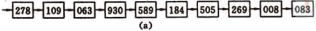
\includegraphics{radixsorta.png}\\
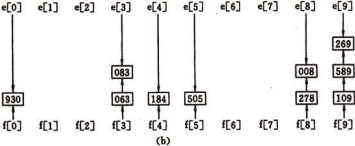
\includegraphics{radixsortb.png}\\
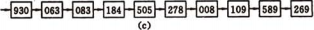
\includegraphics{radixsortc.png}\\
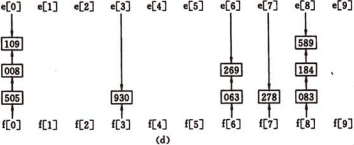
\includegraphics{radixsortd.png}\\
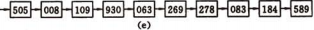
\includegraphics{radixsorte.png}\\
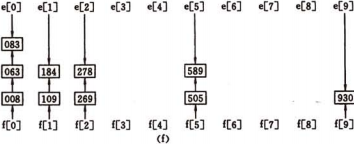
\includegraphics{radixsortf.png}\\
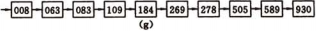
\includegraphics{radixsortg.png}\\
\figcaption{LSD链式基数排序示例}\label{fig:radixsort}
\end{center}

LSD链式基数排序的C语言实现如下。
\begin{Codex}[label=radix_sort.c]
/** @file radix_sort.c
  * @brief LSD链式基数排序.
  * @author soulmachine@gmail.com
  * @date 2013-05-18
  */
#include <stdio.h>  /* for printf() */

/* 关键字基数,此时是十进制*/
#define R 10  /*Radix*/

/**
  *@struct
  *@brief 静态链表结点.
  */
typedef struct static_list_node_t {
    int key; /** 关键字*/
    int link; /** 下一个节点*/
}static_list_node_t;

 /*
  * @brief 打印静态链表.
  * @param[in] a 静态链表数组
  * @return 无
  */
static void static_list_print(const static_list_node_t a[]) {
    int i = a[0].link;
    while (i != 0) {
        printf("%d ", a[i].key);
        i = a[i].link;
    }
}

 /*
  * @brief 获取十进制整数的某一位数字.
  * @param[in] n 整数
  * @param[in] i 第i位
  * @return 整数n第i位的数字
  */
static int get_digit(int n, const int i) {
    int j;
    for(j = 1; j < i; j++) {
        n /= 10;
    }

    return n % 10;
}

/**
  * @brief LSD链式基数排序.
  * @param[in] a 静态链表,a[0]是头指针
  * @param[in] n 待排序元素的个数
  * @param[in] d 最大整数的位数
  * @return 无
  * @note 无
  * @remarks 无
  */
void radix_sort(static_list_node_t a[], const int n, const int d) {
    int i, j, k, current, last;
    int rear[R], front[R];

    for(i = 0; i < n; i++) a[i].link = i + 1;
    a[n].link = 0;
    for(i = 0; i < d; i++) {
        /* 分配*/
        for(j = 0; j < R; j++) front[j] = 0;
        for(current = a[0].link; current != 0;
            current = a[current].link) {
            k = get_digit(a[current].key, i + 1);
            if(front[k] == 0) {
                front[k] = current;
                rear[k] = current;
            } else {
                a[rear[k]].link = current;
                rear[k] = current;
            }
        }

        /* 收集*/
        j = 0;
        while(front[j] == 0) j++;
        a[0].link = current = front[j];
        last = rear[j];
        for(j = j + 1; j < R; j++) {
            if(front[j] != 0) {
                a[last].link = front[j];
                last = rear[j];
            }
        }
        a[last].link = 0;
    }
}

void radix_sort_test(void) {
    static_list_node_t a[] = {{0,0}/* 头指针*/, {278,0}, {109,0}, 
    {63,0}, {930,0}, {589,0}, {184,0}, {505,0}, {269,0}, 
    {8,0}, {83,0}};
    radix_sort(a, 10, 3);
    static_list_print(a);
}
\end{Codex}


\section{总结和比较} %%%%%%%%%%%%%%%%%%%%%%%%%%%%%%

\begin{center}
\tabcaption{各种排序算法的总结和比较}

\vspace{1ex}
\begin{tabular}{lcccc}
\hline
\textbf{排序方法} & \textbf{平均时间} & \textbf{最坏情况} & \textbf{辅助存储} & \textbf{是否稳定}\\
\hline
直接插入排序 & $O(n^2)$ & $O(n^2)$ & $O(1)$ & 是\\
折半插入排序 & $O(n^2)$ & $O(n^2)$ & $O(1)$ & 是\\
希尔排序 & N/A & N/A & $O(1)$ & 否\\
冒泡排序 & $O(n^2)$ & $O(n^2)$ & $O(1)$ & 是\\
快速排序 & $O(n\log_2n)$ & $O(n^2)$ & $O(\log_2n)$ & 否\\
简单选择排序 & $O(n^2)$ & $O(n^2)$ & $O(1)$ & 否\\
堆排序 & $O(n\log_2n)$ & $O(n\log_2n)$ & $O(1)$ & 否\\
二路归并 & $O(n\log_2n)$ & $O(n\log_2n)$ & $O(n)$ & 是\\
基数排序 & $O(d\times (n+R))$ & $O(d\times (n+R))$ & $O(R)$ & 是\\
\hline
\end{tabular}
\end{center}

假设在数组中有两个元素$A_i,A_j,i<j$,即$A_i$在$A_j$之前,且$A_i=A_j$,如果在排序之后,$A_i$仍然在$A_j$的前面,则称这个排序算法是\textbf{稳定}的,否则称这个排序算法是\textbf{不稳定}的。

排序方法根据在排序过程中数据是否完全在内存,分为两大类:\textbf{内部排序}和\textbf{外部排序}。内部排序是指在排序期间数据全部存放在内存;外部排序是指在排序期间所有数据不能同时存放在内存,在排序过程中需要不断在内、外存之间交换。一般说到排序,默认是指内部排序。

